\documentclass[12pt]{article}
\usepackage{MathNotes}

% Table of contents hyperlink setup, needs to be separate for some reason
\usepackage{hyperref}
\hypersetup{
 colorlinks,
 linkcolor=blue
}

\begin{document}

\title{Lie Algebra Notes}
\author{Will Huang}
\maketitle
\tableofcontents

\newpage 

\section{Introduction}
These are my personal notes as I work through Georgi's ``Lie Algebras in Particle Physics." I was assigned this book to skim through at the beginning of my first quantum field theory class to read before we started quantum chromodynamics. Unfortunately, I did not and got rapidly lost in the representation theory. This document is my attempt to fix my past mistakes. The aim is to have some brief notes for each chapter followed by my solutions (right or not) to each exercise. 

\section{Preliminaries}
\subsection{The Complex Plane}
First let's define some notation which are used frequently throughout complex analysis and go over some basic results.

Any complex number can be written in the form $z = x + iy$ where $x, y \in \re$. The components $x$ and $y$ are referred to as the real and imaginary parts, respectively, and denoted
\[ x = \Real{z} \qquad y = \Imag{z} \]
Complex numbers without a real part are called purely imaginary. By plotting the real part of a number on the $x$-axis and the imaginary part on the $y$-axis, we get the complex plane. Thus we can identify $\cx \cong \re^2$. 

The complex conjugate of a complex number $z$ is
\[ \bar z = x - iy \]
Thus we have the formulae
\[ \Real{z} = \frac{z + \bar z}{2} \qquad \Imag{z} = \frac{z - \bar z}{2i} \]
If $z = \bar z$, then it is a real number and if $z = -\bar z$ it is purely imaginary.

The magnitude, or absolute value, of a complex number is
\[ \abs{z} = \sqrt{x^2 + y^2} \]
In the complex plane, this is just the distance from the origin to $z$. From this definition, we have the complex analog to the triangle inequality which is exactly the same.
\[ \abs{z + w} \leq \abs{z} + \abs{w} \]
for all $z, w\in \cx$. We also have
\[ \abs{\Real{z}} \leq \abs{z} \qquad \abs{\Imag{z}} \leq \abs{z} \]

From the triangle inequality, we get two more inequalities
\[ \abs{z} \leq \abs{z - w} + \abs{w} \qquad \abs{w} \leq \abs{z - w} + \abs{z} \]
from which we can prove the ``reverse triangle inequality"
\[ \abs{\abs{z} - \abs{w}} \leq \abs{z - w} \]
\begin{proof}
	Using the triangle inequality, we have
	\[ |z - w| + |w| \geq |z - w + w| = |z| \]
	\[ |z - w| + |z| = |z - w| + |-z| \geq |z - w - z| = |-w| = |w| \]
	
	Rewriting both of these gives
	\[ |z - w| \geq |z| - |w| \qquad |z - w| \geq |w| - |z| = -(|z| - |w|) \]
	Now we note that if $x \geq y$ and $x \geq -y$ then $x \geq |y|$. Thus we arrive at the desired result
	\[ |z - w| \geq \abs{|z| - |w|} \]
\end{proof}

Using the complex conjugate, we can write
\[ \abs{z}^2 = z \bar z \qquad \inv z = \frac{\bar z}{|z|^2} \]
With addition and multiplication defined in the natural way, this shows that $\cx$ is a field i.e. a ring in which every nonzero element has a multiplicative inverse. 

Any complex number can be written in polar form and using Euler's formula we may write
\[ z = re^{i\theta} = r \cos\theta + i r\sin\theta \]
We observe that $r = \abs{z}$, the quantity $\theta$ is referred to as the argument and denoted $\arg z = \theta$. In the complex plane, $r$ is the magnitude and $\theta$ the angle from horizontal. If we have two complex numbers
\[ z = re^{i\theta} \qquad w = se^{i\phi} \]
then multiplication is simply
\[ zw = rse^{u(\theta + \phi)} \]
Thus multiplication in the complex plane is a homothety in $\re^2$.

Now we may discuss more analytical properties of complex numbers, in particular limits and convergence. We should be familiar with these concepts from the real numbers already, we just need carry over them to the complex plane. 

\newpage 
\begin{definition}[Convergence]
	A sequence $\setb{z_1, z_2, \ldots, z_n}$ is said to converge to $w \in \cx$ if 
	\[\lim_{n \to \infty} \abs{z_n - w} = 0 \]
	If the sequence converges, we write
	\[ \lim_{n \to \infty} z_n = w \]
\end{definition}

This is nothing new, since $\cx \cong \re^2$. In fact a sequence of complex numbers converges to a point $w$ if and only if the corresponding points in $\re^2$ converge to the point corresponding to $w$.

\begin{proposition}[Convergence of Complex Numbers]
	A sequence of complex numbers converges to $w$ if and only if their real and imaginary parts converge to $\Real{w}$ and $\Imag{w}$ respectively.
\end{proposition}
\begin{proof}
	Obvious if we think of points in $\cx$ as points in $\re^2$.
\end{proof}

We don't always know what a sequence converges to, so we need another condition to tell us when an arbitrary sequence converges. This condition should be familiar.

\begin{definition}[Cauchy Sequences]
	A sequence $\setb{z_n}$ is Cauchy if 
	\[ \abs{z_n - z_m} \to 0 \text{ as } n,m \to \infty \]
	
	Equivalently, for every $\epsilon > 0$ there exists an integer $N > 0$ such that
	\[ n,m < N \thus |z_n - z_m| < \epsilon \]
\end{definition}

A fundamental result from real analysis is that every Cauchy sequence in $\re$ converges to a real number, that is $\re$ is complete. This is true in the complex plane as well.

\begin{theorem}[Completeness of $\cx$]
	The field of complex numbers $\cx$ is complete, that is every Cauchy sequence of complex numbers will converge to a complex number.
\end{theorem}
\begin{proof}
	A sequence on complex numbers is Cauchy if and only if the real and imaginary parts are both Cauchy. Since $\re$ is complete, we know then that those ``subsequences" will converge to a real number. Thus a Cauchy sequence of complex numbers will converge to a complex number.
\end{proof}

The final preliminary we must cover is the topology of $\cx$, in particular the notion of open sets. As usual, nothing new is being introduced, we are simply bringing over existing constructions and making them work. The remainder of this section is essentially a series of definitions.

Let $z_0 \in \cx$ be some point and $r > 0$, the open disc centered at $z_0$ of radius $r$ is the set
\[ D_r(z_0) = \setb{z \in \cx \mid \abs{z - z_0} < r} \]
Similarly, the closed disc centered at $z_0$ of radius $r$ is the set 
\[ \bar{D_r}(z_0) = \setb{z \in \cx \mid \abs{z - z_0} \leq r} \]
Of note is the unit disc, which has a special notation since it is so useful
\[ \D = \setb{z \in \cx \mid |z| < 1} \]

\begin{definition}[Interior and Limit Points]
	Let $\Omega \subset \cx$, a point $z_0 \in \Omega$ is an interior point if there exists an $r > 0$ such that
	\[ D_r(z_0) \subset \Omega \]
	In words, a point is interior if there exists an open disc around it contained completely within $\Omega$. The set of interior points is called the interior of $\Omega$, usually denoted $\text{int } \Omega$. 
	
	A point $z \in \cx$, not necessarily in $\cx$, is a limit point if there exists a sequence
	\[ \setb{z_n \mid z_n \neq z} \in \Omega \qquad \lim_{n \to \infty} z_n = z \]
	Alternatively, $z$ is a limit point of $\Omega$ if every open disc containing $z$ contains at least one other point of $\Omega$.
\end{definition}

A set is open if it is equal to its interior and closed if its complement is open. 

\begin{proposition}
	A set $\Omega$ is closed if and only if it contains all of its limit points
\end{proposition}
\begin{proof}
	First suppose $\Omega$ is closed and $w$ be a limit point of $\Omega$. Then there exists a sequence $\setb{w_n} \in \Omega$ such that 
	\[ \lim_{n \to \infty} w_n = 0 \]
	
	This means that for every $\epsilon > 0$, there exists an $N > 0$ such that for all $n > N$ we have $|w - w_n| < \epsilon$. Equivalently, for every $r > 0$ the open disc $D_r(w)$ contains a point of $\Omega$. Thus $w$ cannot be in the interior of $\Omega^c$, but $\Omega^c$ is open so $w$ must lie in $\Omega$. 
	
	Conversely suppose $\Omega$ is a set which contains all its limit points. Take some $w \not\in \Omega$ and assume for the sake of contradiction that $w \not\in \text{int } \Omega^c$. In other words, there does not exist an $r > 0$ such that $D_r(w) \subset \Omega^c$. Let $\setb{r_n}$ be any sequence of real number converging to 0, then
	\[ D_{r_n}(w) \cap \Omega \neq \varnothing \]
	
	Let $w_n$ be the (not-necessarily unique) points in each intersection, this is a sequence of points in $\Omega$ which converge to $w$. But $w$ cannot be a limit point of $\Omega$, so we conclude that there must be an open disc around $w$ which lies in $\Omega^c$. Thus $\Omega^c$ is open and $\Omega$ is closed.
\end{proof}

Using this proposition, we can closed any set by adding its limit points. This is known as the closure and denoted $\bar\Omega$.

The boundary of a set $\Omega$ is equal to its closure minus its interior, denoted
\[ \partial \Omega = \bar\Omega - \text{int } \Omega \]
For the open and closed discs, their boundary is the circle
\[ C_r(z_0) = \setb{z \in \cx \mid \abs{z - z_0} = r} \]

A set $\Omega$ is bounded if there exists some $M > 0$ such that $|z| < M$ for all $z \in \Omega$, which implies that $\Omega$ is contained which some large open disc. For bounded sets we define the diameter
\[ \text{diam } \Omega = \sup_{z, w\in \Omega} \abs{z - w} \]

A set is compact if it is closed and bounded.

\begin{theorem}
	A set $\Omega \subset \cx$ is compact if and only if every sequence $\setb{z_n} \in \Omega$ has a subsequence that converges to a point in $\Omega$
\end{theorem}
\begin{proof}
	First let $\Omega$ be compact and let $\setb{z_n} \in \Omega$ be some sequence of points. Consider
	\[ \setb{x_n} = \setb{\Real{z_n}} \in \re \qquad \setb{y_n} = \setb{\Imag{z_n}} \in \re \]
	
	These are both bounded sequences in $\re$ since $\Omega$ is bounded, thus they have a convergence subsequence by the Bolzano–Weierstrass Theorem. Suppose the subsequences converge to $x, y \in \re$ respectively, then we can construct a subsequence of $\setb{z_n}$ which converges to $z = x + iy$. 
	
	Now suppose $\Omega$ is not compact, which means it is either not closed or not bounded (or both!). If $\Omega$ is not closed, then take some point $w \in \bar\Omega \setminus \Omega$. This is a limit point of $\Omega$ and so comes with a sequence $\setb{w_n} \in \Omega$ which converges to it. This means that every convergent subsequence of $\setb{w_n}$ must also converge to $w$. 
	
	If $\Omega$ is not bounded, then we can trivially construct an unbounded sequence. Any subsequence will then never converge. Thus $\Omega$ is compact if and only if every sequence has a convergence subsequence.
\end{proof}

A more familiar condition for compactness is the following

\begin{theorem}
	An open covering is a (not necessarily countable) family of open sets $\setb{U_\alpha}$ such that
	\[ \Omega \subset \bigcup_\alpha U_\alpha \]
	A set $\Omega$ is compact if and only if every open covering of $\Omega$ has a finite subcovering. 
\end{theorem}
\begin{proof}
	Consider points in $\cx$ as points in $\re^2$, then this follows from Heine-Borel.
\end{proof}

When we have nested compact sets, we get an interesting result. This will be very useful as be start diving more deeply into complex analysis.

\begin{proposition}
	Suppose we have a nested sequence of non-empty compact sets in $\cx$
	\[ \Omega_1 \supset \Omega_2 \supset \Omega_3 \supset \cdots \supset \Omega_n \supset \cdots \]
	with the property
	\[ \lim_{n \to \infty} \text{diam } \Omega_n = 0 \]
	Then there exists a unique $w \in \cx$ such that $w \in \Omega_n$ for all $n$.
\end{proposition}
\begin{proof}
	Pick $z_n \in \Omega_n$, then the condition that the diameter converges to 0 means this is a Cauchy sequence, thus it converges to some point $z$. But each set is compact, so the subsequences must converge to $z$ in every set. 
	
	Suppose $w'$ is another point in each $\Omega_n$, then $|w - w'| > 0$ since $w \neq w'$ which violates the assumption that the diameters converge to 0.
\end{proof}

Finally, an open set $\Omega$ is connected if it cannot be expressed in the form
\[ \Omega = \Omega_1 \cup \Omega_2 \]
where $\Omega_1, \Omega_2$ are disjoint nonempty sets. A similar definition applies for closed sets and we call connected sets in $\cx$ regions.

An equivalent and useful definition of connected is as follows: An open set $\Omega$ is connected if and only if any two points in $\Omega$ can be joined by a curve $\gamma$ contained entirely in $\Omega$. This proposition is proved in Exercise 5 below.

\subsection{Complex Functions}
We can now discuss functions defined on sets of complex numbers.

\begin{definition}[Continuous Functions]
	Let $f$ be a function defined on an open complex set $\Omega \to \cx$. We say $f$ is continuous if for every $\epsilon > 0$, there exists a $\delta > 0$ such that 
	\[ |z - z_0| < \delta \thus |f(z) - f(z_0)| < \epsilon \quad \forall z \in \Omega \]
	Equivalently, for every sequence $\setb{z_n} \in \Omega$ which converges to $z_0$, the sequence $\setb{f(z_n)} \in \cx$ must converge to $f(z_0)$.
\end{definition}

We say that a function in continuous on a set if it is continuous at every point of that set. We've previously established that convergence in $\cx$ is identical to that of $\real$, so a complex function is continuous if and only it is continuous if viewed as a function of two real variables. As expected, sum and products of continuous functions will remain continuous in $\cx$.

\begin{theorem}
	A continuous function on a compact set $\Omega$ is bounded and will achieve both a maximum and minimum on $\Omega$. 
\end{theorem}

We now introduce a central idea in complex analysis, something specific to complex functions.

\begin{definition}[Holomorphic Functions]
	Let $f$ be a function $f: \Omega \to \cx$, then $f$ is holomorphic at the point $z_0 \in \Omega$ if the limit
	\[ f'(z_0) = \lim_{h \to 0} \frac{f(z_0 + h) - f(z_0)}{h} \]
	exists where $h \neq 0 \in \cx$ and $z_0 + h \in \Omega$. The second condition is required for the quotient to be defined. This limit is known as the derivative of $f$ at $z_0$.
\end{definition}

We say that $f$ is holomorphic on an open set $\Omega$ if it is holomorphic on every point $z \in \Omega$. We say $f$ is holomorphic on a closed set $C$ if it is holomorphic on some open set which contains $C$. Finally, if $f$ is holomorphic on all of $\cx$, then we say it is entire. The terms regular, complex differentiable, and analytic are sometimes used in place of the term holomorphic.

\begin{example}
	All polynomials are entire,
	\[ p(z) = a_0 + a_1z + a_2z^2 + \cdots + a_nz^n \thus p'(z) = a_1 + 2a_2 z + \cdots + n a_nz^{n-1} \]
	The function $1/z$ is holomorphic on any open set of $\cx$ which does not contain the origin
	\[ f(z) = \frac{1}{z} \thus f'(z) = -\frac{1}{z^2} \]
\end{example}

\begin{example}
	The function $f(z) = \bar z$ is not holomorphic, the limit quotient is
	\[ f'(z) = \lim_{h \to 0} \frac{\bar{z + h} - \bar z}{h} = \lim_{h \to 0} \frac{\bar h}{h} \]
	The final limit does not exist, which we can see by taking $h$ first to be real and then purely imaginary (we get 1 and -1 as limit respectively).
\end{example}

While we won't prove them, it is worth noting that all the standard derivative rules apply to holomorphic functions. By further examining the difference quotient, we see that $f$ is holomorphic at $z_0 \in \Omega$ if and only if there exists a complex number $a$ such that
\[ f(z_0 + h) - f(z_0) - ah = h \psi(h) \qquad \lim_{h \to 0} \psi(h) = 0 \]
where $\psi$ is a function defined for small $|h|$. We see that $a$ then must be $f'(z_0)$ and this formulation shows that $f$ must be continuous if it is holomorphic.

The notion of complex differentiability is very different from the notion of differentiability for a function of two real variables. 

\begin{example}
	Returning to the $f(z) = \bar z$ example, as a map $\re^2 \to \re^2$ this is
	\[ f(x, y) = (x, -y) \]
	and its derivative is a linear map, the Jacobian:
	\[ f'(x, y) = \det \mathbf J_f(x,y) \mqty[x \\ y] = \det \mqty[1 & 0 \\ 0 & -1] \mqty[x \\ y] = (x, -y) \]
	So as a real function, $f$ is infinitely differentiable. But as a complex function, it is not differentiable at all, the existence of a real derivative does not mean $f$ is holomorphic and vice versa.
\end{example}

Consider a general complex function $f = u + iv$ and associate it with a map
\[ F: \re^2 \to \re^2 \qquad F(x, y) = (u(x,y), v(x,y)) \]
We say that this function is differentiable at a point $P_0 = (x_0, y_0)$ if
\[ \lim_{|H| \to 0} \frac{F(P_0 + H) - F(P_0) - J(H)}{|H|} = 0 \]
in which case $J(H)$ is the derivative of $F$ at $P_0$ and is unique. If both $u, v$ are partial differentiable, then the derivative is given by the Jacobian matrix
\[ \mathbf J_F(x, y) = \mqty(\pdv*{u}{x} & \pdv*{u}{y} \\ \pdv*{v}{x} & \pdv*{v}{y}) \]

So when we take a real derivative we get a matrix, but when we take a complex derivative we get a complex number. Ideally, there will be some sort of relationship between the two derivatives. When we take the limit of the difference quotient of a complex function, the result should be independent of path. So we can take two paths, one purely real and the other purely imaginary, to connect the complex derivative to real partial derivatives.
\begin{align*}
	f'(z_0) &= \lim_{h \to 0} \frac{f(z_0 + h) - f(z_0)}{h} \qquad h \in \re \\
	&= \lim_{h_1 \to 0} \frac{f(x_0 + h_1, y_0) - f(x_0, y_0)}{h_1} \\
	&= \pdv{f}{x}\,(z_0) \\
	f'(z_0) &= \lim_{h \to 0} \frac{f(z_0 + h) - f(z_0)}{h} \qquad h \in \cx \\
	&= \lim_{h_2 \to 0} \frac{f(x_0, y_0 + h_2) - f(x_0, y_0)}{ih_2} \\
	&= \frac{1}{i} \pdv{f}{y} \,(z_0) 
\end{align*}
where we write $f(z) = f(x, y)$, $z = x + iy$, $h = h_1 + i h_2$.

If $f$ is holomorphic, then these two expressions must be equal and we find
\[ f'(z) = \pdv{f}{x} = \frac{1}{i} \pdv{f}{y} = -i \pdv{f}{y} \]

Now if we write $f = u + iv$, we find
\[ \pdv{u}{x} + i \pdv{v}{x} = -i \pdv{u}{y} + \pdv{v}{y} \]
By separating out the real and imaginary parts, we get a pair of very special (non-trivial) relationships between partial derivatives which link real and complex derivatives.

\newpage 
\begin{definition}[Cauchy-Riemann Equations]
	Let $f = u + iv$, then if $f$ is holomorphic, $u$ and $v$ satisfy the Cauchy-Riemann equations:
	\[ \pdv{u}{x} = \pdv{v}{y} \qquad \qquad \pdv{u}{y} = -\pdv{v}{x} \]
	When $u,v$ are the real and complex parts of a function, we frequently define the operators
	\[ \pdv{z} = \frac{1}{2} \qty( \pdv{x} + \frac{1}{i} \pdv{y}) \qquad \pdv{\bar z} = \frac{1}{2} \qty( \pdv{x} - \frac{1}{i} \pdv{y}) \]
\end{definition}

The first operator simply averages the two equivalent expressions for $f'(z)$ that we found earlier and the second can is just the complex conjugate. Now we may give the relationship between holomorphic functions and the real derivatives of its real and imaginary components.

\begin{theorem}[Holomorphic vs. Real Differentiable]
	If $f$ is holomorphic at $z_0$, then
	\[ \pdv{f}{\bar z}(z_0) = 0 \qquad f'(z_0) = \pdv{f}{z}(z_0) = 2\pdv{u}{z}(z_0) \]
	If we write $F(x, y) = f(x + iy) = f(z)$, then $F$ is real differentiable
	\[ \det \mathbf J_F(x_0, y_0) = \abs{f'(z_0)}^2\]
	
	Conversely, let $f$ be a function from an open set $\Omega \to \cx$. If $u, v$ are continuously differentiable and satisfy the Cauchy-Riemann equations on $\Omega$, then $f$ is holomorphic on $\Omega$ with derivative
	\[ f'(z) = \pdv{f}{z} \]
\end{theorem}
\begin{proof}
	Write $f = u + iv$, if $f$ is holomorphic then we can use the Cauchy-Riemann equations to write
	\begin{align*}
		\pdv{f}{\bar z} &= \frac{1}{2} \qty( \pdv{f}{x} - \frac{1}{i} \pdv{f}{y} ) \\
		&= \frac{1}{2} \qty( \pdv{u}{x} + i \pdv{v}{x} - \frac{1}{i} \pdv{u}{y} - \pdv{v}{y} ) \\
		&= \frac{1}{2} \qty( \pdv{u}{x} + i \pdv{v}{x} + i\qty(-\pdv{v}{x}) - \pdv{u}{x} ) = 0
	\end{align*}
	
	The other equality follows the same way
	\begin{align*}
	 f' = \pdv{f}{z} &= \frac{1}{2} \qty( \pdv{f}{x} - \frac{1}{i} \pdv{f}{y} ) \\
	 &= \frac{1}{2} \qty( \pdv{u}{x} + i \pdv{v}{x} + \frac{1}{i} \pdv{u}{y} + \pdv{v}{y} ) \\
	 &= \pdv{u}{x} + i \pdv{v}{x} = \pdv{u}{x} + \frac{1}{i} \pdv{u}{y} = 2 \pdv{u}{z}
	\end{align*}
	
	By once again using the Cauchy-Riemann equations,
	\[ \det \mathbf J_F(x_0, y_0) = \pdv{u}{x} \pdv{v}{y} - \pdv{v}{x} \pdv{u}{y} = \qty(\pdv{u}{x})^2 + \qty(\pdv{u}{y})^2 = \abs{2\pdv{u}{z}}^2 = \abs{f'(z_0)}^2 \]
	
	Now conversely suppose that $f = u + iv$ is a complex function defined on an open set. Recall the alternate definition of a derivative and use it to write
	\[ u(x_1 + h_1, y + h_2) - u(x, y) = \pdv{u}{x} h_1 + \pdv{u}{y} h_2 + |h|\psi_1(h) \]
	\[ v(x_1 + h_1, y + h_2) - v(x, y) = \pdv{v}{x} h_1 + \pdv{v}{y} h_2 + |h|\psi_2(h) \]
	where $\psi_i(h) \to 0$ and $h = h_1 + ih_2$. We can combine the two using Cauchy-Riemann equations
	\[ f(z + h) - f(z) = \qty(\pdv{u}{x} - i \pdv{u}{y}) h + |h| \psi(h) \]
	where now $\psi(h) = \psi_1(h) + i\psi(h) \to 0$. This implies $f$ is holomorphic (as we've recovered the derivative definition) and that the derivative is
	\[ f'(z) = \pdv{u}{x} - i \pdv{u}{y} = 2\pdv{u}{z} = \pdv{f}{z} \]
\end{proof}

\newpage 
\subsection{Power Series}
tf is a power series

\newpage 
\subsection{Integration}
tf is an integral

\newpage 
\subsection{Exercises}

% 1
\begin{exercise} \hfill
	\begin{enumerate}[label=\alph*)]
		\item If $|z - z_1| = |z - z_2|$, then we have the set of points equidistant from $z_1, z_2$. On the complex plane this is the line midpoint perpendicular to the line segment connecting $z_1$ and $z_2$. 
		\item If $1/z = \bar z$, then $z\bar z = |z|^2 = 1$. This is a unit circle.
		\item $\Real{z} = 3$ is just a vertical line at $x = 3$.
		\item $\Real{z} > c$ is a vertical region to the right of the vertical line $x = 3$ but not including it. The set $\Real{z} \geq c$ would include that line.
		\item Suppose we decompose each complex number as
		\[ a = a_1 + i a_2 \qquad b = b_1 + i b_2 \qquad z = x + i y \]
		Then the condition becomes
		\[ a_1 x - a_2 y + b_1 > 0 \thus y < \frac{a_1}{a_2} x + \frac{b_1}{a_2} \]
		
		This is the shaded region below a line, not including that line. If $b$ is purely imaginary, then the line will pass through the origin. The line is horizontal if $a$ is purely imaginary and vertical if $a$ is real. If $a$ is zero, then either we shade the entire plane if $b$ has a positive real part or nothing otherwise.
		\item Letting $z = x + iy$, this is the region
		\[ x^2 + y^2 = x + 1 \]
		which is a circle slightly right of center with radius $\sqrt{5}/2$
		\item $\Imag{z} = c$ is a horizontal line at $y = c$.
	\end{enumerate}
\end{exercise}

% 2
\begin{exercise}
	Suppose $z = z_1 + iz_2, w = w_1 + iw_2$, then it is straight-forward to verify
	\begin{align*}
		\vbrack{z,w} &= z_1 w_2 + z_2 w_1 \\
		&= \frac{1}{2}( z_1w_1 - iz_1w_2 + iz_2w_1 + z_2w_2 + z_1w_1 + iz_1w_2 - iz_2w_1 + z_2w_2 ) \\
		&= \frac{1}{2}( (z,w) + (w,z) ) = \frac{1}{2}( (z,w) + \bar{(z,w)} ) \\
		&= \Real{z,w}
	\end{align*}
\end{exercise}

% 3
\begin{exercise}

\end{exercise}

% 4
\begin{exercise}

\end{exercise}

% 5
\begin{exercise}

\end{exercise}

% 6
\begin{exercise}

\end{exercise}

% 7
\begin{exercise}

\end{exercise}

% 8
\begin{exercise}

\end{exercise}

% 9
\begin{exercise}

\end{exercise}

% 10
\begin{exercise}

\end{exercise}

% 11
\begin{exercise}

\end{exercise}

% 12
\begin{exercise}

\end{exercise}

% 13
\begin{exercise}

\end{exercise}

% 14
\begin{exercise}

\end{exercise}

% 15
\begin{exercise}

\end{exercise}

% 16
\begin{exercise}

\end{exercise}

% 17
\begin{exercise}

\end{exercise}

% 18
\begin{exercise}

\end{exercise}

% 19
\begin{exercise}

\end{exercise}

% 20
\begin{exercise}

\end{exercise}

% 21
\begin{exercise}

\end{exercise}

% 22
\begin{exercise}

\end{exercise}

% 23
\begin{exercise}

\end{exercise}

% 24
\begin{exercise}

\end{exercise}

% 25
\begin{exercise}

\end{exercise}

% 26
\begin{exercise}

\end{exercise}
\section{Limits}
\subsection{Introduction to Limits}
Limits form the very backbone of calculus, almost every concept and definition comes from the limit of something else. Intuitively they are quite simple: the limit of a something is simply where is appears to be going. In practice, we need a much more rigorous definition. To see why, we turn to the ancient Greeks.

In around 450 BC, Zeno, as ancient Greek philosophers tended to do, sat around thinking of paradoxes. Here are two of his most famous:
\begin{enumerate}
	\item Atalanta\footnote{Famous figure in Greek mythology} is trying to walk to the end of a path. To walk the entire path she must first walk half the path, then half the remaining path (a quarter), then half the next remaining path (an eigth), then a sixteenth, a thirty-second, etc. Since Atalanta has to walk an infinite number of paths, how can she ever finish walking the path? 
	\item Achilles\footnote{Even more famous figure in Greek mythology} is racing a tortoise\footnote{A very famous figure in fairy tale lore, famously starred in the hit movie ``Tortoise and the Hare"}. To make if fair, he gives the tortoise a head start (say 100m). Once he takes off and covers the first 100m, the tortoise would've meandered a couple more meters. Once he runs the next few meters, the tortoise will cover a few more meters, and so on so forth. So the questions is: If every time Achilles catches up to where the tortoise was prior, the tortoise remains a bit ahead, how will Achilles ever pass the tortoise?
\end{enumerate}

The astute reader may notice that these paradoxes are clearly resolvable. After all, we walk across paths all the time and obviously Achilles will eventually pass the turtle, so why are these so famous? 

The reason why these paradoxes are even talked about now is because they deal with the concept of infinity and infinitesimals (infinitely small distances). In order to have a precise mathematical way of dealing with these, we must invent new mathematics. That new mathematics is Calculus.

To introduce the idea of a limit, let's write the Atalanta (formally known as the Dichotomy) paradox in terms of limits (kind of). For Atalanta, suppose the path is 1m long and she walks at a speed of 1m/s. Then the time taken will be
\[ t = \frac{1}{2} + \frac{1}{4} + \frac{1}{8} + \frac{1}{16} + \cdots \]

Let's try to add up the terms in this sequence, if $n$ is the number of terms we add up
\begin{center}
\begin{tabular}{|c|c|c|c|c|c|c|c|c|c|}
\hline 
n & 1 & 2 & 3 & 4 & 5 & $\cdots$ & 10 & $\cdots$ & $\infty$ \\ 
\hline 
t & 1/2 & 3/4 & 7/8 & 15/16 & 31/32 & $\cdots$ & 1023/1024 & $\cdots$ & 1 \\ 
\hline 
\end{tabular} 
\end{center}

We see that as $n$ gets really, really large, then $t$ gets really close to 1. This makes sense because Atalanta should be able to walk the 1m path in 1s.

With that history lesson out of the way, let's return to the math. Take a simple function, for instance $f(x) = x$, and let's look at how it behaves around $x = 1$. There's two ways we can answer this question:
\begin{enumerate}
	\item Start from the left of the graph and see what happens as we move up to $x = 1$
	\item Start from the right of the graph and see what happens as we move down to $x = 1$
\end{enumerate}

It's pretty obvious in this case, but we see that the graph approaches $y = 1$ regardless of which direction we approach. This idea of seeing what happens when we get close to a value is formalized in the definition of a limit.

\begin{definition}[The Limit]
Let $f(x)$ be a function and $a, L$ some real numbers. If all values of $f(x)$ approach $L$ as $x$ approaches $a$, then we say that $L$ is the limit of the function $f(x)$ as $x$ approaches $a$. In symbols, we write this as
\[ \lim_{x \to a} f(x) = L \]
\end{definition}

\begin{example}
What we got from the previous simple example is that
\[ \lim_{x \to 1} x = 1 \]
\end{example}

A quick and dirty way to evaluate limits is to evaluate a bunch of values progressively closer to the value we wish to look at. If the $y$ values appears to get closer to some number, then that number is probably the limit.

\begin{example}

Consider the function $f(x) = x^2$ and suppose we want to find the limit as $x$ approaches $2$. To evaluate this limit using a table, we compute the following values:

\begin{center}
\begin{tabular}{|c|c|c|c|c|c|c|}
\hline 
x & 1.9 & 1.99 & 1.999 & 2.001 & 2.01 & 2.1 \\ 
\hline 
f(x) & 3.61 & 3.9601 & 3.996001 & 4.004001 & 4.0401 & 4.41 \\ 
\hline 
\end{tabular} 
\end{center}

From looking at this table, we can make an educated guess at the limit
\[ \lim_{x \to 2} x^2 = 4 \]

\end{example}

The method of evaluating limits using a table is very crude and, as we saw, very difficult without some form of computer assistance. Throughout mathematics, it is most common to evaluate limits algebraically. First, we discuss the notion of a one-sided limit.

\newpage 
\begin{definition}[One-Sided Limits]
Let $f(x)$ be a function and $a$ some real number. There are two different one-sided limits:
\begin{itemize}
	\item If $f(x)$ approaches a real number $L$ as $x$, where $x < a$, approaches $a$, then the \textbf{left-sided limit} of $f(x)$ as $x$ approaches $a$ is $L$, or in symbols
	\[ \lim_{x \to a^-} f(x) = L \]
	\item If $f(x)$ approaches a real number $M$ as $x$, where $x > a$, approaches $a$, then the \textbf{right-sided limit} of $f(x)$ as $x$ approaches $a$ is $M$, or in symbols
	\[ \lim_{x \to a^+} f(x) = M \]
\end{itemize}
\end{definition}

\begin{example}
Consider a piece-wise function
\[ f(x) = \begin{cases} 
x & x \leq 0 \\
x^2 + 1 & x > 0
\end{cases} \]

If we approach 0 from the left, we are on the top function. We can plug in 0 directly to find
\[ \lim_{x \to 0^-} f(x) = 0 \]

From the right we are on the bottom function. We can still plug in 0 even though the condition is $x > 0$ because limits are not about what the function actually is, rather it is about what the function is approaching. Thus
\[ \lim_{x \to 0^+} f(x) = 0^2 + 1 = 1 \]

\end{example}

This method of ``plug-and-chug" is generally how most limits will be evaluated. In the rare case that this doesn't work (for instance we end up dividing by zero), we'll need to do some more algebra.

\begin{theorem}[Two-Sided Limits]
The limit of a function $f(x)$ as $x$ approaches $a$ exists if and only if both one-sided limits exist and are equal, that is
\[ \lim_{x \to a} f(x) = \lim_{x \to a^-} f(x) = \lim_{x \to a^+} f(x) \]
\end{theorem}

Thus we cannot conclude that a limit exists unless both the left- and right-handed limits exist and are equal. 

\begin{example}
	Let $a$ and $c$ be any two real numbers, the two most basic limits are
	\[ \lim_{x \to a} c = c \qquad \lim_{x \to a} x = a \]
\end{example}


\begin{example}
	Sometimes the limit does not exist because we try to do something illegal, for instance
	\[ \lim_{x \to -4} \sqrt{x} = \varnothing \]
	because we cannot square root a negative\footnote{Technically we can, but then we would have to work in the complex plane and that requires much more complicated machinery (complex analysis)}
\end{example}

\begin{example}
	Consider a piece-wise function
	\[ f(x) = \begin{cases} 
	\sin(x) & x <= 0 \\ 
	\cos(x) & x > 0 
	\end{cases} \]
	We have the following one-sided limits
	\[ \lim_{x \to 0^-} f(x) = 0 \qquad \lim_{x \to 0^+} f(x)= 1 \]
	Since the two are not equal, the limit of $f(x)$ as $x$ approaches $0$ does not exist.
\end{example}

Sometimes we end up trying to do something illegal when we ``plug-and-chug," but that does not always mean the limit doesn't exist. In some cases infinity (or negative infinity) is a perfectly valid answer\footnote{Though it can be debated if these limits actually exist}. Identifying infinite limits requires a bit of brainpower. The process is similar to making a table of values but we don't actually do it. It's easiest to demonstrate with examples:

\begin{example}
	Consider the function $f(x) = 1/x$ as $x$ approaches 0. From the right side we get smaller and smaller $x$ values, which means that $f(x)$ gets larger and larger. Thus we can write
	\[ \lim_{x \to 0^+} f(x) = \infty \]
	From the left side we also get smaller and smaller values, but negative. Thus rather than get bigger, $f(x)$ gets more and more negative, so we write
	\[ \lim_{x \to 0^-} f(x) = -\infty \]
	Since these two one-sided limits are not the same, the limit does not exist.
\end{example}

\begin{example}
	Now consider the function $f(x) = 1/x^2$. We can use a similar argument from last time, but since the denominator is squared, the function will always be positive. Thus
	\[ \lim_{x \to 0} f(x) = \lim_{x \to 0^-} f(x) = \lim_{x \to 0^+} f(x) = \infty \]
\end{example}

The value of the limit is not the only place where infinity could exist, we may be interested in the behavior of the function as $x$ itself approach positive/negative infinity. Again, we demonstrate with an example:

\begin{example}
	Consider the function $f(x) = 1/x$ again. Suppose we want to know the limit as $x$ goes to infinity. To do this, we think about what happens as $x$ gets larger and larger. Clearly $f(x)$ would get smaller and smaller as the denominator grows, so
	\[ \lim_{x \to \infty} f(x) = 0 \]
	Similarly, we can show that
	\[ \lim_{x \to -\infty} f(x) = 0 \]
\end{example}

Limits with infinity gives us a way to find asymptotes without having to draw a graph.
\begin{theorem}
	Let $f(x)$ be a function and $a$ a real number. The line $x = a$ is a vertical asymptote if both one-sided limits are positive or negative infinity. In symbols
	\[ \lim_{x \to a^-} f(x) = \pm \infty \qquad \lim_{x \to a^+} f(x) = \pm \infty \]
	Note that this does not mean the limit itself is defined as we say in the case of $f(x) = 1/x$. 
	
	The line $y = a$ is a horizontal asymptote if the limit as $x$ goes to positive or negative infinity is $a$.
	\[ \lim_{x \to -\infty} f(x) = a \qquad \text{ or } \qquad \lim_{x \to \infty} f(x) = a \]
\end{theorem}

\begin{example}
	Let's find all asymptotes for the following function
	\[ f(x) = \frac{1}{1 - x} + 3 \]
	First we do the horizontal asymptotes
	\[ \lim_{x \to -\infty} f(x) = \lim_{x \to \infty} f(x) = 3 \]
	so $y = 3$ is a horizontal asymptote for this function.
	
	It's a bit harder to see the vertical asymptotes right away, but a good way to find them is to look for ``divide by zeros" and then evaluate the limits. In this case we consider $x = 1$
	\[ \lim_{x \to 1^-} = \infty \qquad \lim_{x \to 1^+} = - \infty \]
	Notice that the left handed limit is positive infinity this time. This is because when $x < 1$, the denominator is very small but positive. When dealing with infinities, it is very important to make sure you have the right one.
\end{example}

If we are given a graph of a function, we can evaluate limits visually by examining the behavior of the graph. For instance if we wanted to evaluate a left-handed limit, we can place our pencil a bit to the left of the point and trace the line up to that point. The height that we appear to be approaching is the limit. Remember: the limit is what the function appears to approaching, not what it actually is.\footnote{If it helps, you may think of limits as "It is not the destination that matters, but the journey"}

\begin{example} 
Consider the following graph of a function $f(x)$
\begin{center}
	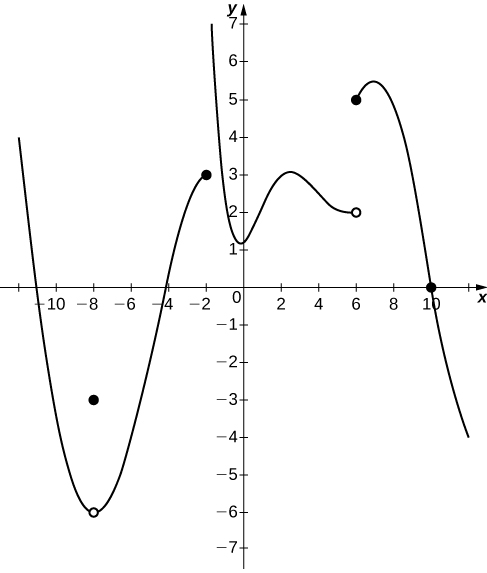
\includegraphics[scale=1]{images/Figure 2.2.1.jpg}
\end{center}

At $x = -8$, we see that from the left and the right we are approaching the same value. The fact that $f(-8) = -3$ does not matter, the limits are
\[ \lim_{x \to -8^-} f(x) = \lim_{x \to -8^+} f(x) = \lim_{x \to -8} f(x) = -6 \]

At $x = -2$ the graph has different behavior depending on if we are on the left or right. If we trace the graph coming from the left, we will approach $y = -2$ and in fact this is also the value of $f(-2)$. If we come from the right then we go straight up to $+ \infty$. Thus
\[ \lim_{x \to -2^-} f(x) = 3 \qquad \lim_{x \to -2^+} = \infty \qquad \lim_{x \to -2} = \varnothing \]

The remaining two interesting points, $x = 6$ and $x = 10$, will be left as an exercise to the sufficiently motivated and astute reader.
\end{example}

\newpage 
\subsection{Techniques for Limits}

Now that we've brute forced our way through a couple limits, it is time to find a way to use those previous results to evaluate new limits. A lot of these laws/rules may seem obvious but it is important to state them nonetheless.

\begin{theorem}[Properties of Limits]
	Let $f(x)$ and $g(x)$ be functions, $a$ a real number, and suppose $f,g$ have the following limits
	\[ \lim_{x \to a} f(x) = L \qquad \lim_{x \to a} g(x) = M \]
	
	Then we have the following properties, let $c$ be a constant
	\begin{align*}
		\lim_{x \to a} f(x) \pm g(x) &= \lim_{x \to a} f(x) \pm \lim_{x \to a} g(x) = L \pm M \\
		\lim_{x \to a} f(x)g(x) &= \lim_{x \to a} f(x) \cdot \lim_{x \to a} g(x) = L \cdot M \\
		\lim_{x \to a} cf(x) &= c \cdot \lim_{x \to a} f(x) = c \cdot L \\
		\lim_{x \to a} \frac{f(x)}{g(x)} &= \frac{\lim_{x \to a} f(x)}{\lim_{x \to a} g(x)} = \frac{L}{M} \qquad \text{ if $M \neq 0$} \\
		\lim_{x \to a} (f(x))^n &= \qty(\lim_{x \to a} f(x))^n = L^n \\
		\lim_{x \to a} \sqrt[n]{f(x)} &= \sqrt[n]{\lim_{x \to a} f(x)} = \sqrt[n]{L}
	\end{align*}
	
	The last result holds for all $x$ if $n$ is odd and all $x \geq 0$ if $n$ is even (these also happen to be the domains of $\sqrt[n]{x}$ for odd/even $n$).
\end{theorem}

These laws give the ``plug and chug" strategy a more mathematical reasoning. Since we know the two basic limits
\[ \lim_{x \to a} c = c \qquad \lim_{x \to a} x = a \]
we can use the limit laws to manipulate them into the function we are interested in. 

\begin{example}
	Consider the function
	\[ f(x) = \frac{x^2 + 3x - 10}{x^3 - 2x} \]
	
	The using the basic limits, we can evaluate the limit
	\[ \lim_{x \to 2} f(x) = \frac{2^2 + 3 \cdot 2 - 10}{2^3 - 2 \cdot 2} = \frac{0}{4} = 0 \]
\end{example}

It is worth noting that these laws all apply the one-sided limits as well.

There are many tricks to evaluating limits, we'll cover a few of the most common ones in the ensuing exercises.
\begin{example}
	Consider the function
	\[ f(x) = \frac{x^2 + 2x - 3}{x^2 - 1} \]
	
	If we tried to evaluate the limit as $x$ approaches 1, then we would end up dividing by zero. To avoid this we must first factor the top and bottom
	\[ f(x) = \frac{(x + 3)(x - 1)}{(x + 1)(x - 1)} = \frac{x + 3}{x + 1} \]
	Now we see that since a term cancels, we can use the limit laws to evaluate
	\[ \lim_{x \to 1} f(x) = \frac{1 + 3}{1 + 1} = 2 \]
\end{example}

\begin{example}
	When working with square roots it is common to get a function of the form
	\[ f(x) = \frac{\sqrt{x + 1} - 1}{x} \]
	
	If we tried to evaluate the limit as $x$ approaches 0 it would appear to seem that we are stuck. Furthermore there is nothing to factor, so what is there left to do? It turns out that we can use the fact that $x^2 - a^2 = (x + a)(x - a)$ change the fraction. This is known as multiplying by the conjugate, lets see it in action:
	\begin{align*}
		f(x) &= \frac{\sqrt{x + 1} - 1}{x} \cdot \qty(\frac{\sqrt{x + 1} + 1}{\sqrt{x + 1} + 1}) = \frac{(\sqrt{x + 1})^2 - 1^2}{x(\sqrt{x + 1} + 1)} \\
		&= \frac{x + 1 - 1}{x(\sqrt{x + 1} + 1)} = \frac{x}{x(\sqrt{x + 1} + 1)}\\
		&= \frac{1}{\sqrt{x + 1} + 1}
	\end{align*}
	
	This sort of algebraic manipulation is allowed because at the end of the day, all we did was multiply by 1. With the function in this form, we can now evaluate the limit
	\[ \lim_{x \to 0} f(x) = \frac{1}{\sqrt{0 + 1} + 1} = \frac{1}{2} \]
\end{example}

\begin{example}
	When evaluating limits, one should always try to simplify the function as much as possible before preceding. Consider the function
	\[ f(x) = \frac{1}{x} - \frac{3}{x(x + 3)} \]
	
	If we tried to evaluate the limit as $x$ goes to 0, we may be tempted to either say it does not exist or is an asymptote due to the $1/x$. But if we took the time to simply, we find
	\[ f(x) = \frac{x + 3}{x(x + 3)} - \frac{3}{x(x + 3)} = \frac{x}{x(x + 3)} = \frac{1}{x + 3} \]
	Now we can evaluate
	\[ \lim_{x \to 0} f(x) = \frac{1}{0 + 3} = \frac{1}{3} \]
\end{example}

For more complicated limits we may sometimes use the squeeze (or sandwich) theorem when applicable.
\begin{theorem}[Squeeze Theorem]
	Let $f(x), g(x), h(x)$ be functions defined for all $x \neq a$ in an open interval containing $a$. If
	\[ f(x) \leq g(x) \leq h(x) \]
	The their limits obey
	\[ \lim_{x \to a} f(x) \leq \lim_{x \to a} g(x) \leq \lim_{x \to a} h(x) \]
	
	In particular if
	\[ \lim_{x \to a} f(x) = \lim_{x \to a} h(x) = L \]
	then it must be the case that
	\[ \lim_{x \to a} g(x) = L \]
\end{theorem}

To see how we may use this theorem to solve otherwise impossible limits, consider the following example.

\begin{example}
	Suppose we have a function
	\[ f(x) = x \cos(\frac{1}{x}) \]
	and we wish to evaluate the limit as $x$ goes to 0. We can't use the limit laws because then we'd be dividing by zero, so instead we note that
	\[ -1 \leq \cos(x) \leq 1 \qquad \text{ and so } \qquad -x \leq f(x) \leq x \]
	
	It doesn't matter what's inside the cosine because it will always be between -1 and +1. Thus we just need to compute
	\[ \lim_{x \to 0} -x = 0 \qquad \lim_{x \to 0} x = 0 \]
	and we are able to conclude, using the squeeze theorem,
	\[ \lim_{x \to 0} f(x) = 0 \]
\end{example}

Note that in order to actually get a limit out of the squeeze theorem, the limit on both sides of the inequality must be the same. If they are different, then the squeeze limit does not tell us anything.

\begin{Optional}[Important Trigonometric Limits]
For this subsection I will use without proof the following limits\footnote{A geometric proof of the first limit using the squeeze theorem is provided in the textbook and the second can be found by multiplying by the conjugate}
\[ \lim_{x \to 0} \frac{\sin(x)}{x} = 1 \qquad \lim_{x \to 0} \frac{1 - \cos x}{x} = 0\]

Let's see how we can use these two limits to evaluate a deceptively difficult limit

\begin{example}
	Consider the function
	\[ f(x) = \frac{\sin^2(3x)}{\sin(2x)} \]
	
	We want to evaluate the limit as $x$ approaches $0$. At first glance, we don't really see much that we can do. After all, both the numerator and denominator goes to zero. However, before we give up and quit math forever, we notice that there is one (indeed the only) thing to do: rewrite the numerator. 
	\[ f(x) = \frac{1 - \cos^2(3x)}{\sin(2x)} = \frac{(1 + \cos(3x))(1 - \cos(3x))}{\sin(2x)} \]
	
	We now remember that we've seen part of this numerator before, it's the same numerator in the limit we first introduced! But we're missing the denominator, furthermore the function instead the cosine is $x$, not $3x$. To fix this, we turn to the old trick: multiply by 1. This also fixes the sine in the denominator
	\begin{align*}
		f(x) &= \frac{(1 + \cos(3x))(1 - \cos(3x))}{\sin(2x)} \cdot \qty(\frac{2x}{2x}) \cdot \qty(\frac{3x}{3x}) \\
		&= \qty(\frac{2x}{\sin(2x)}) \cdot \qty(\frac{1 - \cos(3x)}{3x}) \cdot \qty(\frac{2x(1 + \cos(3x))}{3x}) \\
		&= \frac{2}{3} \qty(\frac{1}{\sin(2x)/2x}) \qty(\frac{1 - \cos(3x)}{3x}) (1 + \cos(3x))
	\end{align*}
	Now we can evaluate the limit
	\[ \lim_{x \to 0} f(x) = \frac{2}{3} \cdot \frac{1}{1} \cdot 0 \cdot (1 + 0) = 0 \]
\end{example}

\end{Optional}

\newpage 
\subsection{Continuity}

% Definition of continuity
% Types of discontinuity
% Interval continuity + examples
% Limit composition
% Intermediate value theorem

\newpage 
\subsection{Hard Topic: Precise Definition of a Limit}

% Introduction to epsilon delta
% Examples
% Proving a limit law
% Very hard example/proof

\end{document}